\subsection{Lumped capacitance}
    \begin{minipage}{0.39 \linewidth}
        Idea: The temperature in a body is almost uniform, so we can assume it to be uniform.
        Temperature within body will now be $T(t)$ instead of $T(t, x, y, z)$.
        That means, the temperature difference inside the body $\Delta T_i = T_{s, 1} - T_{s, 2}$ must be much smaller than the temperature difference outside the body $\Delta T_o = T_{s, 2} - T_{\infty}$.
    \end{minipage}
    \begin{minipage}{0.59 \linewidth}
        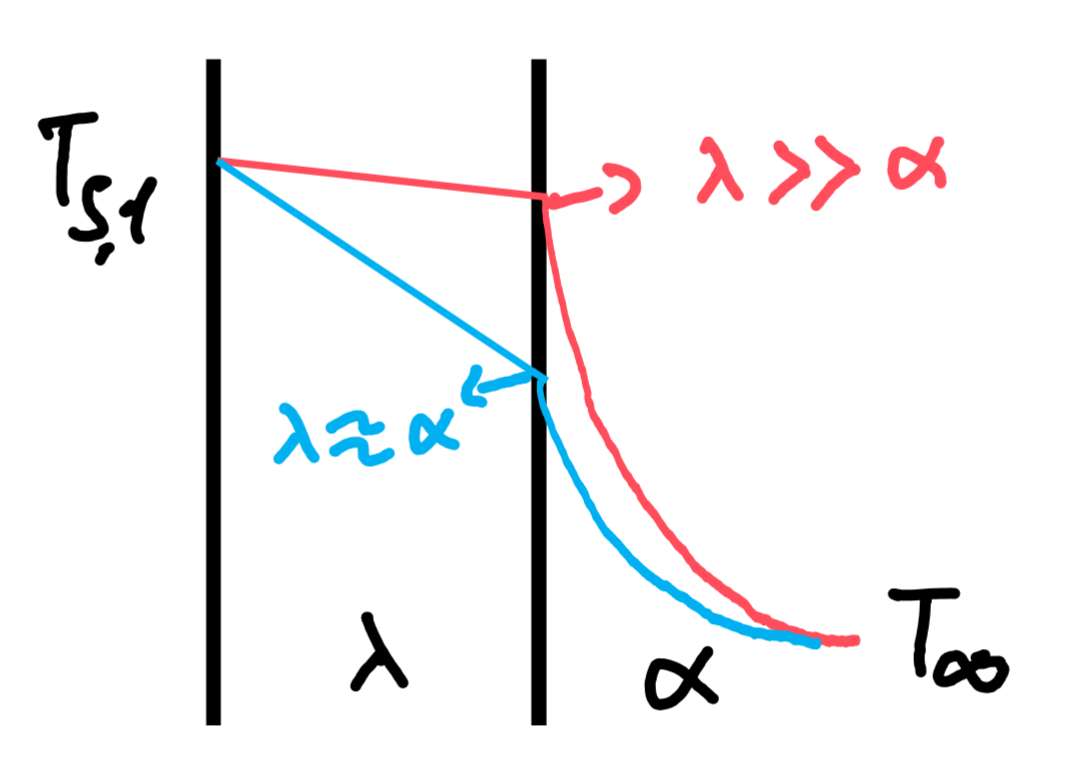
\includegraphics[width = \linewidth]{src/images/lumped_cap.png}
    \end{minipage}

    \begin{empheq}{align*}
        \dot{q} = \frac{\lambda A}{L} (T_{s, 1} - T_{s, 2}) = \alpha A (T_{s, 2} - T_{\infty})\\
        \Rightarrow \frac{(T_{s, 1} - T_{s, 2})}{(T_{s, 2} - T_{\infty})} = \frac{\alpha L}{\lambda} = Bi\\
        L_{\text{cylinder}} = \frac{r}{2} \quad \quad L_{\text{sphere}} = \frac{r}{3}
    \end{empheq}